\documentclass[11pt,a4paper,landscape]{article}
\usepackage[landscape,margin=1.5cm]{geometry}
\usepackage{tikz}
\usepackage[T1]{fontenc}
\usepackage{xcolor}
\usepackage{multicol}
\usepackage{array}
\usepackage{tabularx}
\usepackage{graphicx}
\usepackage{amssymb}
\usepackage{pifont}
\usepackage{helvet}
\renewcommand{\familydefault}{\sfdefault}

% Define colors for each letter
\definecolor{letterM}{HTML}{C2185B}  % Pink
\definecolor{letterN}{HTML}{1565C0}  % Blue
\definecolor{letterO}{HTML}{E65100}  % Orange
\definecolor{letterP}{HTML}{7B1FA2}  % Purple
\definecolor{lightgray}{HTML}{E0E0E0}
\definecolor{tracegray}{HTML}{CCCCCC}

% Remove page numbers
\pagestyle{empty}

% Custom commands for tracing letters
\newcommand{\tracebox}[1]{%
    \tikz[baseline=(char.base)]{
        \node[draw=tracegray, line width=1pt, minimum width=2cm, minimum height=2.5cm, inner sep=0pt] (char) {%
            \textcolor{tracegray!70}{\fontsize{48}{52}\selectfont #1}%
        };
    }%
}

\newcommand{\emptybox}{%
    \tikz[baseline=-0.5ex]{
        \node[draw=lightgray, line width=1pt, minimum width=2cm, minimum height=2.5cm, inner sep=0pt] {};
    }%
}

\newcommand{\lettercard}[3]{%
    \begin{tikzpicture}
        \node[draw=#2, line width=2pt, rounded corners=8pt, minimum width=3cm, minimum height=3.5cm, fill=#2!10] (card) {};
        \node at (card.center) {\textcolor{#2}{\fontsize{60}{65}\selectfont #1}};
        \node[anchor=south] at (card.south) {\small\textbf{#3}};
    \end{tikzpicture}%
}

\newcommand{\lettergrid}[1]{%
    \tikz[baseline=-0.5ex]{
        \node[draw=lightgray, minimum size=1.2cm, font=\Large\bfseries] {#1};
    }%
}

\begin{document}

% ============ PAGE 1: Meet the Letters ============
\begin{center}
{\fontsize{28}{32}\selectfont\textbf{Letter Review: M, N, O, P}}\\[0.3cm]
{\large Name: \underline{\hspace{8cm}} \hspace{2cm} Date: \underline{\hspace{4cm}}}
\end{center}

\vspace{0.5cm}

\begin{center}
{\Large\textbf{Meet the Letters!}}\\[0.5cm]

\begin{tabular}{cccc}
\lettercard{Mm}{letterM}{Mouse} &
\lettercard{Nn}{letterN}{Nest} &
\lettercard{Oo}{letterO}{Orange} &
\lettercard{Pp}{letterP}{Pig}
\end{tabular}
\end{center}

\vspace{0.8cm}

\begin{center}
{\Large\textbf{Trace the Uppercase Letters}}\\[0.3cm]
{\small Trace each letter, then write it yourself.}\\[0.5cm]

\begin{tabular}{cccccccc}
\tracebox{M} & \emptybox & \hspace{0.5cm} &
\tracebox{N} & \emptybox & \hspace{0.5cm} &
\tracebox{O} & \emptybox \\[0.5cm]
\multicolumn{2}{c}{\textcolor{letterM}{\textbf{M is for Mouse}}} & &
\multicolumn{2}{c}{\textcolor{letterN}{\textbf{N is for Nest}}} & &
\multicolumn{2}{c}{\textcolor{letterO}{\textbf{O is for Orange}}}
\end{tabular}

\vspace{0.5cm}

\begin{tabular}{cc}
\tracebox{P} & \emptybox \\[0.5cm]
\multicolumn{2}{c}{\textcolor{letterP}{\textbf{P is for Pig}}}
\end{tabular}
\end{center}

\newpage

% ============ PAGE 2: Lowercase Tracing ============
\begin{center}
{\fontsize{24}{28}\selectfont\textbf{Trace the Lowercase Letters}}\\[0.3cm]
{\small Trace each letter, then write it yourself.}
\end{center}

\vspace{0.5cm}

\begin{center}
\begin{tabular}{cccccccc}
\tracebox{m} & \emptybox & \hspace{0.5cm} &
\tracebox{n} & \emptybox & \hspace{0.5cm} &
\tracebox{o} & \emptybox \\[1cm]
\tracebox{p} & \emptybox & & & & & &
\end{tabular}
\end{center}

\vspace{1cm}

\begin{center}
{\Large\textbf{Writing Practice}}\\[0.3cm]
{\small Write each letter 5 times on the lines below.}\\[0.5cm]

\begin{tabular}{lcl}
\textcolor{letterM}{\fontsize{36}{40}\selectfont M m} & \hspace{0.5cm} &
\tikz{\draw[lightgray, line width=1pt] (0,0) -- (18cm,0);} \\[0.8cm]

\textcolor{letterN}{\fontsize{36}{40}\selectfont N n} & \hspace{0.5cm} &
\tikz{\draw[lightgray, line width=1pt] (0,0) -- (18cm,0);} \\[0.8cm]

\textcolor{letterO}{\fontsize{36}{40}\selectfont O o} & \hspace{0.5cm} &
\tikz{\draw[lightgray, line width=1pt] (0,0) -- (18cm,0);} \\[0.8cm]

\textcolor{letterP}{\fontsize{36}{40}\selectfont P p} & \hspace{0.5cm} &
\tikz{\draw[lightgray, line width=1pt] (0,0) -- (18cm,0);} \\
\end{tabular}
\end{center}

\newpage

% ============ PAGE 3: Matching Activity ============
\begin{center}
{\fontsize{24}{28}\selectfont\textbf{Match the Letters}}\\[0.3cm]
{\small Draw a line to match the uppercase letter to the lowercase letter.}
\end{center}

\vspace{1cm}

\begin{center}
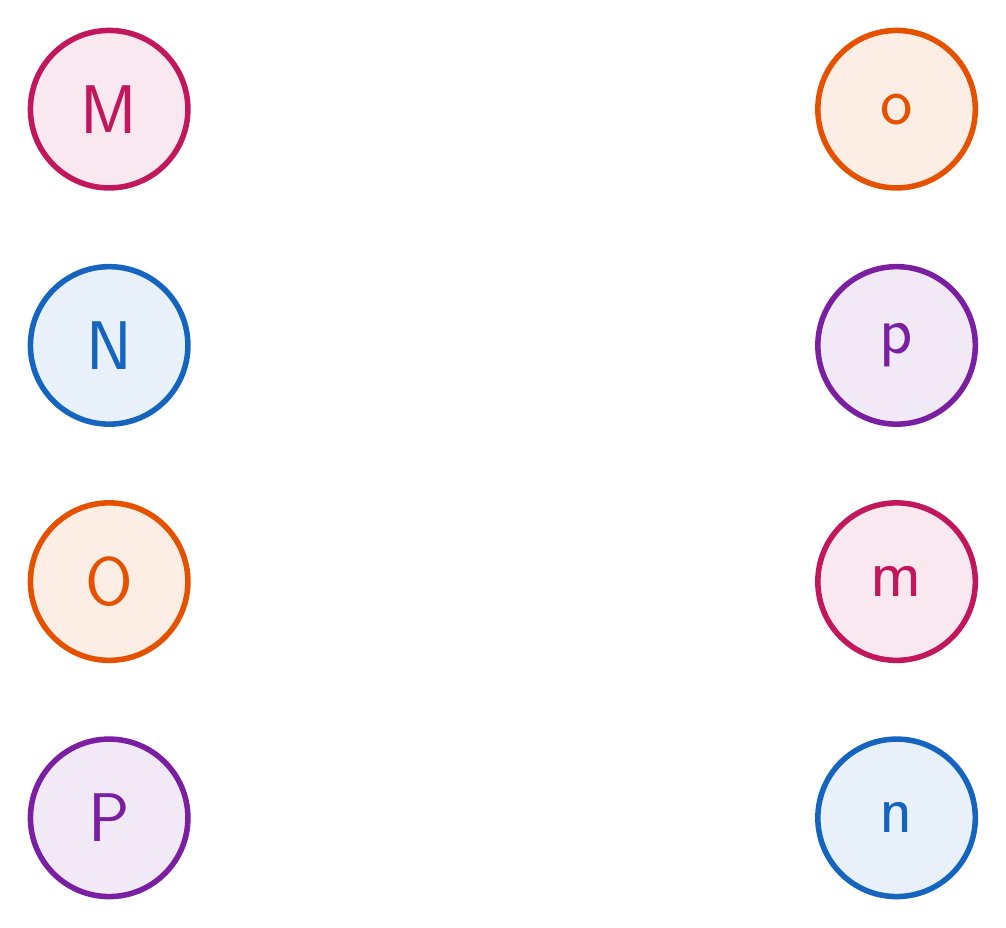
\begin{tikzpicture}
    % Left column - uppercase
    \node[draw=letterM, line width=2pt, circle, minimum size=2cm, fill=letterM!10] at (0,6) {\textcolor{letterM}{\fontsize{36}{40}\selectfont M}};
    \node[draw=letterN, line width=2pt, circle, minimum size=2cm, fill=letterN!10] at (0,3) {\textcolor{letterN}{\fontsize{36}{40}\selectfont N}};
    \node[draw=letterO, line width=2pt, circle, minimum size=2cm, fill=letterO!10] at (0,0) {\textcolor{letterO}{\fontsize{36}{40}\selectfont O}};
    \node[draw=letterP, line width=2pt, circle, minimum size=2cm, fill=letterP!10] at (0,-3) {\textcolor{letterP}{\fontsize{36}{40}\selectfont P}};

    % Right column - lowercase (shuffled)
    \node[draw=letterO, line width=2pt, circle, minimum size=2cm, fill=letterO!10] at (10,6) {\textcolor{letterO}{\fontsize{36}{40}\selectfont o}};
    \node[draw=letterP, line width=2pt, circle, minimum size=2cm, fill=letterP!10] at (10,3) {\textcolor{letterP}{\fontsize{36}{40}\selectfont p}};
    \node[draw=letterM, line width=2pt, circle, minimum size=2cm, fill=letterM!10] at (10,0) {\textcolor{letterM}{\fontsize{36}{40}\selectfont m}};
    \node[draw=letterN, line width=2pt, circle, minimum size=2cm, fill=letterN!10] at (10,-3) {\textcolor{letterN}{\fontsize{36}{40}\selectfont n}};
\end{tikzpicture}
\end{center}

\vspace{1cm}

\begin{center}
{\Large\textbf{Match Letters to Pictures}}\\[0.3cm]
{\small Write the correct letter (M, N, O, or P) next to each word.}\\[0.5cm]

\begin{tabular}{|c|c|c|c|}
\hline
\rule{0pt}{1.5cm} \Large\textbf{Moon} & \underline{\hspace{2cm}} &
\rule{0pt}{1.5cm} \Large\textbf{Orange} & \underline{\hspace{2cm}} \\
\hline
\rule{0pt}{1.5cm} \Large\textbf{Nest} & \underline{\hspace{2cm}} &
\rule{0pt}{1.5cm} \Large\textbf{Pencil} & \underline{\hspace{2cm}} \\
\hline
\end{tabular}
\end{center}

\newpage

% ============ PAGE 4: Beginning Sounds ============
\begin{center}
{\fontsize{24}{28}\selectfont\textbf{Beginning Sounds}}\\[0.3cm]
{\small Circle the letter that each word starts with.}
\end{center}

\vspace{0.8cm}

\begin{center}
\begin{tabular}{|p{5cm}|c|c|c|c|p{5cm}|c|c|c|c|}
\hline
\textbf{Word} & M & N & O & P & \textbf{Word} & M & N & O & P \\
\hline
\rule{0pt}{1.2cm}\Large \textbf{MONKEY} & $\bigcirc$ & $\bigcirc$ & $\bigcirc$ & $\bigcirc$ &
\Large \textbf{NOSE} & $\bigcirc$ & $\bigcirc$ & $\bigcirc$ & $\bigcirc$ \\
\hline
\rule{0pt}{1.2cm}\Large \textbf{OCTOPUS} & $\bigcirc$ & $\bigcirc$ & $\bigcirc$ & $\bigcirc$ &
\Large \textbf{PENGUIN} & $\bigcirc$ & $\bigcirc$ & $\bigcirc$ & $\bigcirc$ \\
\hline
\rule{0pt}{1.2cm}\Large \textbf{NOODLES} & $\bigcirc$ & $\bigcirc$ & $\bigcirc$ & $\bigcirc$ &
\Large \textbf{MANGO} & $\bigcirc$ & $\bigcirc$ & $\bigcirc$ & $\bigcirc$ \\
\hline
\rule{0pt}{1.2cm}\Large \textbf{PIZZA} & $\bigcirc$ & $\bigcirc$ & $\bigcirc$ & $\bigcirc$ &
\Large \textbf{OWL} & $\bigcirc$ & $\bigcirc$ & $\bigcirc$ & $\bigcirc$ \\
\hline
\end{tabular}
\end{center}

\vspace{1cm}

\begin{center}
{\Large\textbf{Write the Beginning Letter}}\\[0.3cm]
{\small Look at each word. Write the first letter in the box.}\\[0.5cm]

\begin{tabular}{cccc}
\fbox{\rule{1.2cm}{0pt}\rule{0pt}{1.2cm}} \textbf{\_ouse} &
\fbox{\rule{1.2cm}{0pt}\rule{0pt}{1.2cm}} \textbf{\_est} &
\fbox{\rule{1.2cm}{0pt}\rule{0pt}{1.2cm}} \textbf{\_range} &
\fbox{\rule{1.2cm}{0pt}\rule{0pt}{1.2cm}} \textbf{\_ig} \\[0.8cm]

\fbox{\rule{1.2cm}{0pt}\rule{0pt}{1.2cm}} \textbf{\_et} &
\fbox{\rule{1.2cm}{0pt}\rule{0pt}{1.2cm}} \textbf{\_ilk} &
\fbox{\rule{1.2cm}{0pt}\rule{0pt}{1.2cm}} \textbf{\_en} &
\fbox{\rule{1.2cm}{0pt}\rule{0pt}{1.2cm}} \textbf{\_ctopus} \\
\end{tabular}
\end{center}

\newpage

% ============ PAGE 5: Letter Hunt ============
\begin{center}
{\fontsize{24}{28}\selectfont\textbf{Letter Hunt!}}\\[0.3cm]
{\small Find and circle all the letters \textcolor{letterM}{\textbf{M}}, \textcolor{letterN}{\textbf{N}}, \textcolor{letterO}{\textbf{O}}, and \textcolor{letterP}{\textbf{P}} in the grid below.}
\end{center}

\vspace{0.5cm}

\begin{center}
\begin{tabular}{|c|c|c|c|c|c|c|c|c|c|c|c|}
\hline
\rule{0pt}{1cm}\Large A & \Large\textcolor{letterM}{M} & \Large B & \Large\textcolor{letterN}{N} & \Large C & \Large\textcolor{letterO}{O} & \Large D & \Large\textcolor{letterP}{P} & \Large E & \Large\textcolor{letterM}{M} & \Large F & \Large\textcolor{letterN}{N} \\
\hline
\rule{0pt}{1cm}\Large\textcolor{letterN}{N} & \Large G & \Large\textcolor{letterO}{O} & \Large H & \Large\textcolor{letterP}{P} & \Large I & \Large\textcolor{letterM}{M} & \Large J & \Large\textcolor{letterN}{N} & \Large K & \Large\textcolor{letterO}{O} & \Large L \\
\hline
\rule{0pt}{1cm}\Large\textcolor{letterO}{O} & \Large\textcolor{letterM}{M} & \Large\textcolor{letterP}{P} & \Large\textcolor{letterN}{N} & \Large A & \Large B & \Large\textcolor{letterO}{O} & \Large C & \Large\textcolor{letterP}{P} & \Large D & \Large\textcolor{letterM}{M} & \Large E \\
\hline
\rule{0pt}{1cm}\Large\textcolor{letterP}{P} & \Large F & \Large\textcolor{letterM}{M} & \Large G & \Large\textcolor{letterN}{N} & \Large H & \Large\textcolor{letterO}{O} & \Large I & \Large\textcolor{letterP}{P} & \Large J & \Large\textcolor{letterM}{M} & \Large K \\
\hline
\rule{0pt}{1cm}\Large\textcolor{letterM}{M} & \Large L & \Large\textcolor{letterN}{N} & \Large\textcolor{letterO}{O} & \Large\textcolor{letterP}{P} & \Large A & \Large B & \Large\textcolor{letterM}{M} & \Large C & \Large\textcolor{letterN}{N} & \Large D & \Large\textcolor{letterO}{O} \\
\hline
\rule{0pt}{1cm}\Large\textcolor{letterN}{N} & \Large E & \Large\textcolor{letterO}{O} & \Large F & \Large\textcolor{letterM}{M} & \Large G & \Large\textcolor{letterP}{P} & \Large H & \Large\textcolor{letterN}{N} & \Large I & \Large\textcolor{letterO}{O} & \Large J \\
\hline
\end{tabular}
\end{center}

\vspace{0.5cm}

\begin{center}
{\large How many did you find?}\\[0.3cm]
\begin{tabular}{cccc}
\textcolor{letterM}{\fontsize{28}{32}\selectfont M} &
\textcolor{letterN}{\fontsize{28}{32}\selectfont N} &
\textcolor{letterO}{\fontsize{28}{32}\selectfont O} &
\textcolor{letterP}{\fontsize{28}{32}\selectfont P} \\
\fbox{\rule{1.5cm}{0pt}\rule{0pt}{1cm}} &
\fbox{\rule{1.5cm}{0pt}\rule{0pt}{1cm}} &
\fbox{\rule{1.5cm}{0pt}\rule{0pt}{1cm}} &
\fbox{\rule{1.5cm}{0pt}\rule{0pt}{1cm}} \\
\end{tabular}
\end{center}

\newpage

% ============ PAGE 6: Review Quiz ============
\begin{center}
{\fontsize{24}{28}\selectfont\textbf{Letter Review Quiz}}\\[0.3cm]
{\small Circle the correct answer for each question.}
\end{center}

\vspace{0.5cm}

\begin{multicols}{2}

\textbf{1. Which letter does MOUSE start with?}\\[0.3cm]
\begin{tabular}{cccc}
\fbox{\Large\textbf{ M }} & \fbox{\Large\textbf{ N }} & \fbox{\Large\textbf{ O }} & \fbox{\Large\textbf{ P }}
\end{tabular}

\vspace{0.6cm}

\textbf{2. Which letter does NEST start with?}\\[0.3cm]
\begin{tabular}{cccc}
\fbox{\Large\textbf{ M }} & \fbox{\Large\textbf{ N }} & \fbox{\Large\textbf{ O }} & \fbox{\Large\textbf{ P }}
\end{tabular}

\vspace{0.6cm}

\textbf{3. Which letter does ORANGE start with?}\\[0.3cm]
\begin{tabular}{cccc}
\fbox{\Large\textbf{ M }} & \fbox{\Large\textbf{ N }} & \fbox{\Large\textbf{ O }} & \fbox{\Large\textbf{ P }}
\end{tabular}

\vspace{0.6cm}

\textbf{4. Which letter does PIG start with?}\\[0.3cm]
\begin{tabular}{cccc}
\fbox{\Large\textbf{ M }} & \fbox{\Large\textbf{ N }} & \fbox{\Large\textbf{ O }} & \fbox{\Large\textbf{ P }}
\end{tabular}

\vspace{0.6cm}

\textbf{5. Which is the lowercase of M?}\\[0.3cm]
\begin{tabular}{cccc}
\fbox{\Large\textbf{ n }} & \fbox{\Large\textbf{ m }} & \fbox{\Large\textbf{ p }} & \fbox{\Large\textbf{ o }}
\end{tabular}

\columnbreak

\textbf{6. Which letter does MOON start with?}\\[0.3cm]
\begin{tabular}{cccc}
\fbox{\Large\textbf{ M }} & \fbox{\Large\textbf{ N }} & \fbox{\Large\textbf{ O }} & \fbox{\Large\textbf{ P }}
\end{tabular}

\vspace{0.6cm}

\textbf{7. Which letter does PENCIL start with?}\\[0.3cm]
\begin{tabular}{cccc}
\fbox{\Large\textbf{ M }} & \fbox{\Large\textbf{ N }} & \fbox{\Large\textbf{ O }} & \fbox{\Large\textbf{ P }}
\end{tabular}

\vspace{0.6cm}

\textbf{8. Which is the lowercase of N?}\\[0.3cm]
\begin{tabular}{cccc}
\fbox{\Large\textbf{ m }} & \fbox{\Large\textbf{ o }} & \fbox{\Large\textbf{ n }} & \fbox{\Large\textbf{ p }}
\end{tabular}

\vspace{0.6cm}

\textbf{9. Which letter does OCTOPUS start with?}\\[0.3cm]
\begin{tabular}{cccc}
\fbox{\Large\textbf{ M }} & \fbox{\Large\textbf{ N }} & \fbox{\Large\textbf{ O }} & \fbox{\Large\textbf{ P }}
\end{tabular}

\vspace{0.6cm}

\textbf{10. Which is the lowercase of P?}\\[0.3cm]
\begin{tabular}{cccc}
\fbox{\Large\textbf{ o }} & \fbox{\Large\textbf{ p }} & \fbox{\Large\textbf{ m }} & \fbox{\Large\textbf{ n }}
\end{tabular}

\end{multicols}

\vspace{0.8cm}

\begin{center}
{\Large\textbf{Great Job!}}\\[0.3cm]
{\large Write your favorite letter from M, N, O, P:}\\[0.5cm]
\fbox{\rule{3cm}{0pt}\rule{0pt}{2.5cm}}
\end{center}

\end{document}
